% create the 4-stage graph of covariant Lyapunov vector algorithm
% use package tikz
% By Xiong
% 
% use the following command to generate the pdf
% pdflatex --jobname=cLv-f1 cLv.tex

\documentclass{article}
\usepackage{graphicx}
\usepackage{tikz}
\usetikzlibrary{calc}
\usetikzlibrary{decorations.markings}
\usetikzlibrary{decorations.pathreplacing}

\tikzset{
  big arrow/.style={
    decoration={markings,mark=at position 0.5 with {\arrow[scale=1.5,blue]{#1}}},
    postaction={decorate},
    shorten >=0.4pt},
  big arrow/.default=>
}

\newcommand{\ssp}{u}

\pgfrealjobname{cLv}

\begin{document}

\beginpgfgraphicnamed{cLv-f1}
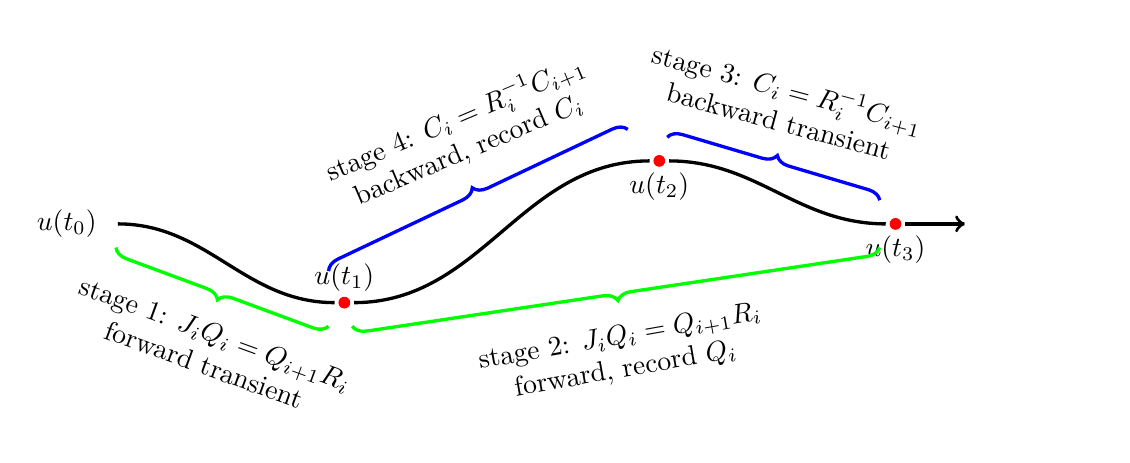
\begin{tikzpicture}
  \node (n1) at (0,0) {};
  \node (n2) at (3,-1) {};
  \node (n3) at (7,0.8){};
  \node (n4) at (10,0) {};
  \node (n5) at (11,0){};
  \node (n6) at (12.5,0){};
  
  \draw[very thick, black] (n1) node[left=0.2pt](){$\ssp(t_0)$}
  to[out=0, in=180] (n2) node[fill, red, circle, inner sep=1.5pt](m1){} 
  node[above=0.2pt](){$\ssp(t_1)$}
  to[out=0, in=180] (n3) node[fill, red, circle, inner sep=1.5pt](m2){} 
  node[below=0.2pt](){$\ssp(t_2)$}
  to[out=0, in=180] (n4) node[fill, red, circle, inner sep=1.5pt](m3){} 
  node[below=0.2pt](){$\ssp(t_3)$}
  to[out=0, in=180] (n5);
  
  \draw[very thick, black, ->] (n4) -- (n5);
  
  \draw[very thick, green, decorate,
  decoration={brace,amplitude=5pt,mirror}] 
  ($(n1)+(0.1,-0.3)$) -- ($(n2)+(-0.2,-0.3)$)
  node[black, midway, below=10pt, align=center,rotate=-20]
  {stage 1: $J_iQ_i=Q_{i+1}R_{i}$ \\ forward transient};

  \draw[very thick, green, decorate,
  decoration={brace,amplitude=5pt,mirror}] 
  ($(n2)+(0.1,-0.3)$) -- ($(n4)+(-0.2,-0.3)$)
  node[black, midway, below=10pt, align=center,rotate=10]
  {stage 2: $J_iQ_i=Q_{i+1}R_{i}$ \\ forward, record $Q_i$};

  \draw[very thick, blue, decorate,
  decoration={brace,amplitude=5pt}] 
  ($(n3)+(0.1,0.3)$) -- ($(n4)+(-0.2,0.3)$)
  node[black, midway, above=10pt, align=center,rotate=-15]
  {stage 3: $C_i=R^{-1}_{i}C_{i+1}$ \\ backward transient};

  \draw[very thick, blue, decorate,
  decoration={brace,amplitude=5pt}] 
  ($(n2)+(-0.2,0.4)$) -- ($(n3)+(-0.4,0.4)$)
  node[black, midway, above=10pt, align=center,rotate=23]
  {stage 4: $C_i=R^{-1}_{i}C_{i+1}$ \\backward, record $C_i$};

\end{tikzpicture}
\endpgfgraphicnamed

\end{document}